\chapter{Aplicaciones}
En este capítulo se abordan aplicaciones del Álgebra Lineal  en dos temas considerados de mucho interés como son  la resolución de ecuaciones difrenciales y la aproximación de funciones. 
Los sistemas de ecuaciones diferenciales surgieron para analizar cuantitativamente determinados sistemas físicos. En el campo de la astronomía, y contemplando los  principios físicos como las leyes del movimiento de Newton y la ley de gravitación, el problema matemático  al estudiar el movimiento de dos o más cuerpos, (moviéndose cada uno bajo la acción gravitatoria de los otros) es el de resolver un sistema de ecuaciones diferenciales ordinarias. Por otro lado, el estudio de la teoría de aproximación de funciones también es de importancia fundamental. Comprende dos tipos generales de problemas: uno se refiere a la
búsqueda de la función óptima que pueda  utilizarse  para representar un
conjunto de datos y fue tratado en el Capítulo $4$, en la aproximación por mínimos cuadrados. En este capítulo nos ocuparemos del problema que se presenta cuando  una función se da de
manera explícita, pero se quiere encontrar un tipo más simple de ella, por ejemplo un polinomio, que  sirva para determinar  valores aproximados de la función dada.

\section{Ecuaciones diferenciales}\index{Ecuaciones diferenciales}
Muchas leyes de la física, química, biología y economía se expresan en términos de \textit{ecuaciones diferenciales}, es decir ecuaciones que comprenden funciones y sus derivadas. En esta sección veremos que es posible aplicar el álgebra lineal para resolver ciertos sistemas de ecuaciones diferenciales.
Una de las ecuaciones diferenciales más simple es 
\begin{equation}
  y^\prime=ay
  \label{71}
  \end{equation}
  donde $y=f(x)$ es una función desconocida que se debe determinar, $y^\prime=\frac{dy}{dx}$ es su derivada y $a$ es una constante. La Ec.(\ref{71}) tiene infinitas soluciones, las cuales son funciones de la forma
  \begin{equation}
  y=ce^{ax}
  \label{72}
  \end{equation}
  donde $c$ es una constante arbitraria. Estas funciones son soluciones de $y^\prime=ay$, dado que 
  \begin{equation}
  y^\prime=cae^{ax}=ay
  \label{73}
  \end{equation}
  A la Ec.(\ref{72}) se le da el nombre de \textit{solución general} de $y^\prime=ay$
  
  Con frecuencia el problema físico que genera una ecuación diferencial impone alguna condición que permite hallar una solución única a partir de la solución general. Por ejemplo, si se requiere que la solución de $y^\prime=ay$ satisfaga que $y=3$ cuando $x=0$, entonces al sustituir en la solución general Ec.(\ref{73}), se obtiene un valos para $c$:
  \begin{equation}
  3=c  e^{0}=c
  \label{74}
  \end{equation}
  
  Por lo tanto, $y=3 e^{ax}$ es la única solución de $y^\prime=ay$ que satisface la condición agregada, que se conoce como \textit{condición inicial}. Al problema de resolver una ecuación diferencial sujeta a una condición inicial se denomina \textit{problema de valor inicial}.
  
  Dado ahora un sistema de ecuaciones diferenciales, por ejemplo, 
  \begin{eqnarray}
  y^\prime_1&=&3y_1 \nonumber\\
  y^\prime_2&=&-2y_2\nonumber\\
  y^\prime_3&=&5y_3 \nonumber\\
  \label{75}
  \end{eqnarray} 
  se desea hallar la solución del sistema que satisface las condiciones iniciales $y_1(0)=1$, $y_2(0)= 4$ y $y_3(0)=-2$.
  En forma matricial, se tiene  
  \begin{equation}
  Y^\prime=\left(\begin{array}{ccc} 3 & 0  & 0  \\0 & -2 & 0 \\0  & 0 & 5
\end{array}
 \right)Y
 \label{76}
  \end{equation}
  donde $Y=(y_1, y_2, y_3)^T$.
  Debido a que cada ecuación comprende sólo una función desconocida, se puede resolver cada una de las ecuaciones  por separado. De la Ec.(\ref{72}) se obtiene
  \begin{eqnarray*}
  y_1&=&c_1e^{3x} \nonumber\\
  y_2&=&c_2e^{-2x}\nonumber\\
  y_3&=&c_3e^{5x} \nonumber\\
  \end{eqnarray*} 
  A partir de las condiciones iniciales dadas, se obtiene
  \begin{eqnarray}
 1= y_1(0)&=&c_1e^{0}=c_1\nonumber\\
  4=y_2(0)&=&c_2e^{0}=c_2\nonumber\\
  -2=y_3(0)&=&c_3e^{0}=c_3 \nonumber\\
  \label{77}
  \end{eqnarray}
  de modo que la solución que satisface las condiciones iniciales es
  \[
  y_1=e^{3x}, \quad y_2=4e^{-2x},  \quad y_3=-2e^{5x}.
  \]
 El sistema de este ejemplo fue fácil de resolver porque cada ecuación comprendía solo una función desconocida, y fue ese el caso porque la matriz de coeficientes  (\ref{76}) es diagonal. 
 Para resolver el caso cuando la matriz no es diagonal es posible hacer una sustitución para $Y$, $Y=SU$ que conduzca a un nuevo sistema con una matriz diagonal de los coeficientes; y una vez resuelto este sistema más sencillo, se usa esa solución para determinar la del sistema original.
 Si se hacen las sustituciones $Y=PU$ e $Y^\prime=PU^\prime$ en el sistema original 
   \[
  Y^\prime=AY
  \]
  y se supone que $S$ tiene inversa, se obtiene 
  \[
  SU^\prime=A(SU)
  \]
  o bien, 
  \[
  U^\prime=(S^{-1}AS)U
  \]
  o bien,
  \[
  Y^\prime=DY
  \]
  donde $D=S^{-1}AS$. Está claro cómo elegir $S$ si se desea que la nueva mtriz de los coeficientes $D$ sea diagonal. Se debe elegir $S$ como la matriz que diagonalice a $A$.
  El procedimiento para resolver un sistema 
  \[
  Y^\prime=AY
  \]
 con una matriz $A$ diagonalizable lo veremos con un ejemplo.
  
Suponga que una partícula se mueve en un campo de fuerzas plano y que
su vector de posición $X$ satisface $X^\prime	 = AX$  y $X(0) = X_0$, donde
\[
  Y^\prime=\left(\begin{array}{cc} 4 & -5  \\-2 & 1 
\end{array}
 \right)Y
  \]
las condiciones iniciales $x_1(0)=2$.$9$, $x_2(0)= 2$.$6$
Se desea resolver este problema de valor inicial, y trazar la trayectoria de la partícula para $t \ge 0$.
La matriz $A$ de los coeficientes del sistema es 
\[
 \left(\begin{array}{cc} 4 & -5  \\-2 & 1 
\end{array}
 \right).
  \]
 Como se analizó en la Sección \ref{Subespacios invariantes}
 a partir de $Det(A-\lambda I)=0$, se obtienen los autovalores de la matriz, $\lambda_1= 6$ y $\lambda_2= -1$. Los autovectores correspondientes son $\Vec{v}_1=(-5,2)^T$ y $\Vec{v}_2=(1,1)^T$.
 
 De ahí que la matriz 
\[
 S=\left(\begin{array}{cc} -5& 1  \\2 & 1 
\end{array}
 \right)
  \]
diagonaliza a $A$ y 
\[
 D=S^{-1}A S=\left(\begin{array}{cc} 6& 0  \\0 & -1 
\end{array}
 \right).
  \]
  Por lo tanto, la sustitución $X=SU$ y $X'=SU^\prime$
  conduce al nuevo sistema diagonal
  \[
 U^\prime=DU=\left(\begin{array}{cc} 6& 0  \\0 & -1 
\end{array}
 \right)U.
  \]
 De acuerdo a (\ref{72}), si $U=(u_1,u_2)^t$, la solución de este sistema es 
 \begin{eqnarray*}
  u_1&=&c_1e^{6t} \nonumber\\
  u_2&=&c_2e^{-t}\nonumber\\
\end{eqnarray*} 
  y la ecuación $X=SU$ proporciona la solución para $X$
 \[
 X=  \left(\begin{array}{c} x_1  \\x_2 
\end{array}
 \right) =            \left(\begin{array}{cc} -5 & 1  \\2 & 1 
\end{array}
 \right) \left(\begin{array}{c} c_1e^{6t}  \\c_2e^{-t}
\end{array}
 \right)    
  \]
o bien
\begin{eqnarray*}
  x_1&=&-5 c_1e^{6t}+ c_2e^{-t} \nonumber\\
  x_2&=&2 c_1e^{6t}+ c_2e^{-t}\nonumber\\
\end{eqnarray*} 
  
Si se sustituyen las condiciones iniciales, se obtiene $c_1 = −3/70$  y $c_2 = 188/70$,
de modo que la solución que satisface las condiciones iniciales es 
\begin{eqnarray*}
  x_1&=&15/70e^{6t}+ 188/70e^{-t} \nonumber\\
  x_2&=&-6/70e^{6t}+ 188/70e^{-t}\nonumber\\
\end{eqnarray*} 

%\bigskip

\begin{figure}
    \centering
    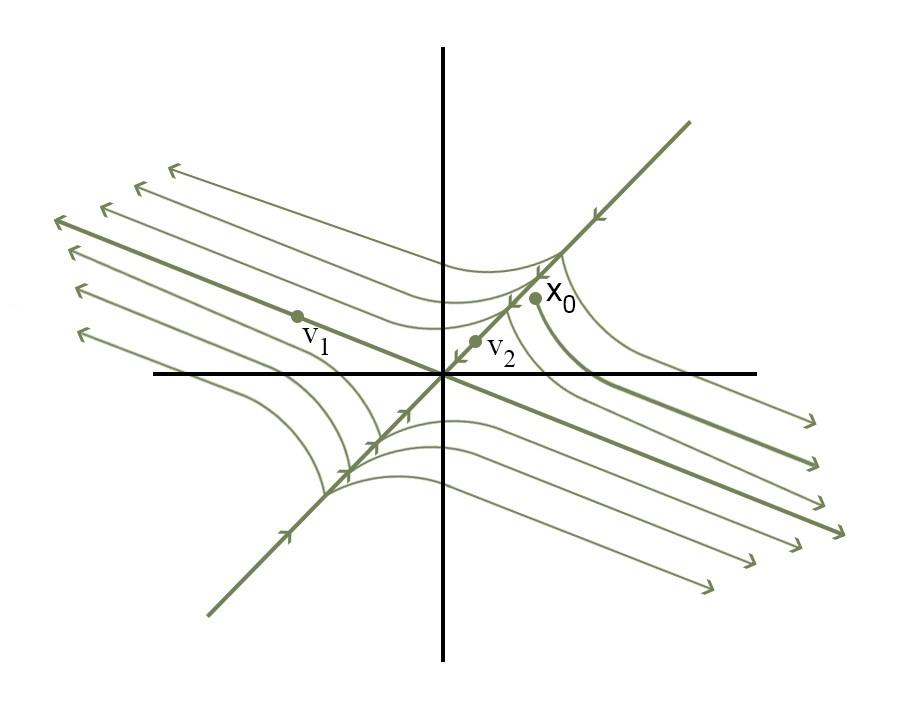
\includegraphics[width=0.7\textwidth]{Pictures/fig.43.jpg}
    \caption{El origen es un punto silla}
    \label{357}
\end{figure} 

 %\begin{example}
Las trayectorias de $X$ se muestran en la Figura  \ref{357}.
Al origen se le llama punto silla del sistema dinámico porque algunas
trayectorias se aproximan primero al origen y luego cambian de dirección y luego se alejan de
él.
Se presenta un punto silla siempre que la matriz $A$ tiene valores propios tanto positivos
como negativos. La dirección de mayor repulsión es la línea que pasa por $\Vec{v}_1$ y $\Vec{0}$
correspondiente al valor propio positivo. La dirección de mayor atracción es la línea que
pasa por $\Vec{v}_2$ y $\Vec{0}$, correspondiente al valor propio negativo.


\bigskip


% agregar un ejemplo para no diagonalizable ej 4 pag 601 del grossman

\index{Caffarelli, Luis Ángel}
\begin{parchment}[Luis Ángel Caffarelli] {Nacido el 8 de diciembre de 1948 en Buenos Aires. Es el principal experto mundial en problemas de frontera libre para ecuaciones diferenciales en derivadas parciales no lineales. También es famoso por sus contribuciones a la ecuación Monge-Ampere y más en general ecuaciones completamente no lineales. Recientemente se ha interesado por los problemas de homogeneización.
En 2023 la Academia Noruega de Ciencias le concedió el Premio Abel, el cuál es semejante al nobel en matemáticas, puesto que éste último no cuenta con distinciones para esta rama del conocimiento. \cite{LuisC} }
\end{parchment}


\bigskip

\section{Problemas de aproximación de funciones.}\index{Aproximación de funciones.}

En muchas aplicaciones se tiene interés en encontrar la mejor aproximación posible sobre un intervalo, para una función $f$, por medio de otra función que pertenece a alguna clase especificada; por ejemplo:

\begin{itemize}
\item  la mejor aproximación posible para $e^x$ en $[0,1]$ por medio de un polinomio de la forma $a_0+a_1x + a_2 x^2$.
\item  la mejor aproximación posible para $sen( \pi x)$ en $[-1,1]$ por medio de una función de la forma $a_0+a_1e^x + a_2 e^{2x}+ a_3 e^{3x}$.

\item  la mejor aproximación posible para $  \left| x   \right|$ en $[0,2 \pi]$ por medio de una función de la forma $a_0+a_1 sen(x) + a_2 sen(2x)+ b_1 cos(x) + b_2 cos(2x)$.


\end{itemize} 


\bigskip

En cada uno de esos ejemplos las funciones de aproximación pertenecen a un subespacio del espacio vectorial $C[a,b]$  (funciones continuas en $[a,b]$), es decir que se está buscando \textit{la mejor aproximación}  utilizando funciones de un subespacio  $W$ de $C[a,b]$. Intuitivamente, la mejor aproximación posible en $[a,b]$ será aquella que produzca el menor error. Si se desea aproximar en un solo punto $x_0$, el error al aproximar $f(x)$ con $g(x)$ estaría dado por $ \left| f(x_0)-g(x_0)   \right|$ (desviación entre $f$ y $g$ en $x_0$). Si se desea la mejor aproximación en un intervalo, se necesita medir el error global de la aproximación $g(x)$. Una medida posible se obtiene integrando la desviación $\left| f(x)-g(x)   \right|$ sobre todo el intervalo; es decir,
\begin{eqnarray}
 \int_a^b {\left| f(x)-g(x)   \right|dx}
 \label{80}
 \end{eqnarray}
 
 Geométricamente (\ref{80}) es el área entre las gráficas de $f(x)$ y $g(x)$ sobre el intervalo $[a,b]$; mayor el área, mayor será el error global.
 Aunque es natural, y geométricamente atractiva, la presencia del valor absoluto hace que se utilice más frecuentemente otra medida del error, conocida como \textit{error cuadrático medio }, definido por 
 \begin{eqnarray}
 ECM=\int_a^b {\left| f(x)-g(x)   \right|^2dx}
 \label{81}
 \end{eqnarray}
 
 La ventaja adicional del ECM es que puede escribirse a partir de la teoría de espacios vectoriales con producto interno (ver Ejemplo \ref{PRODINTL2}). 
 
 Considerando el producto interior 
 \begin{eqnarray}
 (f,g)=\int_a^b {f(x)g(x)dx}
 \label{82}
 \end{eqnarray}
 sobre el espacio vectorial $C[a,b]$, el error cuadrático medio
 \begin{eqnarray}
 ECM=\|f-g\|^2=(f-g,f-g)=\int_a^b{\left| f(x)-g(x)   \right|^2dx}
 \label{83}
 \end{eqnarray}
 es el cuadrado de la distancia entre $f$ y $g$. La aproximación  $g$ en $W$ que minimiza el error cuadrático medio es el vector $g$ en $W$ \textit{más próximo}  a $f$ con el producto interno (\ref{82}). Por lo que vimos en el Teorema \ref{TPOr},  $g$ es la proyección ortogonal de $f$ sobre el subespacio $W$. Entonces, si $f$ es una función continua sobre $[a,b]$ y $W$ es un espacio con dimensión finita de $C[a,b]$, la función $g$ en $W$ que minimiza el error cuadrático medio Ec.(\ref{81}) es $g=P_W f$, que se conoce como \textit{aproximación de los mínimos cuadrados para $f$ en $W$.}
 
 
 \subsection{Series de Fourier}
 
 Una función de la forma
 \begin{eqnarray}
  f(x)=c_0 + c_1 cos(x) + c_2 cos(2x) +  \cdots  + c_n cos(nx)  \nonumber\\
       + d_1 sen(x) + d_2 sen(2x) \cdots  + c_n sen(nx) 
       \label{84}
  \end{eqnarray} 
  se conoce como \textit{polinomio trigonométrico}; si $c_n$ y $d_n$   no son ambos nulos, entonces se dice que $f(x)$ tiene \textit{orden} n.

  \bigskip
  
\begin{example}
  \[
  f(x)=5 + cos(x) - 3 cos(2x) + 7 sen(4x)
       \]
       es un polinomio trigonométrico.  $c_0=5$, $c_1=1$, $c_2=-3$, $d_1=d_2=d_3=0$ y $d_4=7$
de orden $4$.
\end{example}

\bigskip

Por la expresión (\ref{84}) los polinomios trigonométricos de orden $n$ o menos son combinaciones lineales de 
\begin{eqnarray}
  1, \quad cos(x) \quad cos(2x), \quad cos(nx)  \quad  sen(x), \quad sen(2x) \cdots  \quad sen(nx) 
       \label{85}
  \end{eqnarray} 
  y forman un subespacio $W$ del espacio vectorial de funciones continuas; generado por las $2n+1$ funciones de (\ref{85}). Se puede demostrar que estas funciones son linealmente independientes y, como consecuencia, forman una base para $W$.
  
Si se desea hallar una aproximación para una función continua $f(x)$ sobre el intervalo $[-\pi, \pi]$ o $[0, 2\pi]$ por medio de un polinomio trigonométrico de orden $n$ o menor se deberá calcular la proyección ortogonal de $f$ sobre $W$. Para hallar esa proyección ortogonal (Teorema \ref{TPOr}), se deberá encontrar una base ortonormal $g_0$, $g_1$, $g_2$, $\cdots$, $g_{2n}$ para $W$ y luego utilizar la fórmula
\begin{equation}
P_W( f)= (f,g_0)g_0 + (f, g_1)g_1 +  \cdots (f, g_{2n})g_{2n}
 \label{86}
  \end{equation}
  
 Es posible obtener una base ortonormal para $W$ aplicando el método de Gram-Schmidt  a la base (\ref{85}) usando el producto interno (\ref{80}).
 Esto conduce a la base ortonormal
 \begin{eqnarray}
  g_0= \frac{1}{\sqrt{2\pi}}, \quad g_1= \frac{1}{\sqrt{\pi}}   cos(x),  \quad  g_1= \frac{1}{\sqrt{\pi}} cos(2x),\nonumber\\
  \cdots, \quad g_n= \frac{1}{\sqrt{\pi}}  cos(nx),   \quad g_{n+1}= \frac{1}{\sqrt{\pi}} sen(x), \nonumber\\
  \cdots  \quad g_{n+1}= \frac{1}{\sqrt{\pi}}   sen(nx) \nonumber\\
       \label{87}
  \end{eqnarray} 
  
  Si se introduce la notación 
  \begin{eqnarray}
  a_0= \frac{2}{\sqrt{2\pi}}(f,g_0), \quad a_1= \frac{1}{\sqrt{\pi}}(f,g_1)), \cdots \quad  a_n= \frac{2}{\sqrt{2\pi}}(f,g_n),\nonumber\\
  \quad b_1= \frac{1}{\sqrt{\pi}}(f,g_{n+1}), \cdots \quad  b_n= \frac{2}{\sqrt{2\pi}}(f,g_{2n}),
   \label{88}
  \end{eqnarray} 
  
  Reemplazando en  la Ec.(\ref{86}), se obtiene
  \begin{equation}
P_W (f)= \frac{a_0}{2}+ \left[ a_1 cos(x)+ \cdots + a_n cos(nx)   \right] + \left[ b_1 sen(x)+ \cdots + b_n sen(nx)   \right]
 \label{89}
  \end{equation}
  
 Los números $a_0$, $a_1$, $\cdots$,  $a_n$, $b_1$, $\cdots$,  $b_n$ se denominan \texit{coeficientes de Fourier de $f$}.  \index{Coeficientes de Fourier}

 \bigskip
 
 \begin{example}
 
 Se desea hallar la aproximación de mínimos cuadrados de $f(x)$,  
 \begin{eqnarray*}
    f(x)=  
\left \{ \begin{array}{11}
    -1 &  \mbox{cuando $-\pi \leq x \leq 0$},  \\
    1  & \mbox{cuando $0 < x \leq \pi$}
\end{array}
\end{eqnarray*}

\bigskip

en $[-\pi, \pi]$ por medio de un polinomio trigonométrico de orden $2$ o menor.

\bigskip


\begin{eqnarray*}
 a_0= \frac{1}{2 \pi} \int_{-\pi}^{\pi} f(x)dx = \frac{1}{2 \pi}(  \int_{-\pi}^{0} -1 dx+\int_{0}^{\pi} -1 dx )=\frac{1}{2 \pi}(-\pi  + \pi)=0
 \label{99}
 \end{eqnarray*}
 \begin{eqnarray*}
 b_1= \frac{1}{\pi} \int_{-\pi}^{\pi} f(x)sen(x)dx = \frac{1}{\pi} ( \int_{-\pi}^{0} - sen(x)dx   + \int_{0}^{\pi} sen(x) dx =\frac{4}{\pi}
 \label{929}
 \end{eqnarray*}
 
 \bigskip
 
 El resto de los coeficientes son nulos, así que la mejor aproximación a $f(x)$ (por medio de un polinomio trigonométrico de orden $2$ o menor) es,
 \[
 f(x)\approx  \frac{4}{\pi} sen(x)
 \]
La función y su aproximación se muestran en la  Figura \ref{Fourier1}.
\end{example}


\bigskip

\begin{figure}
    \centering
    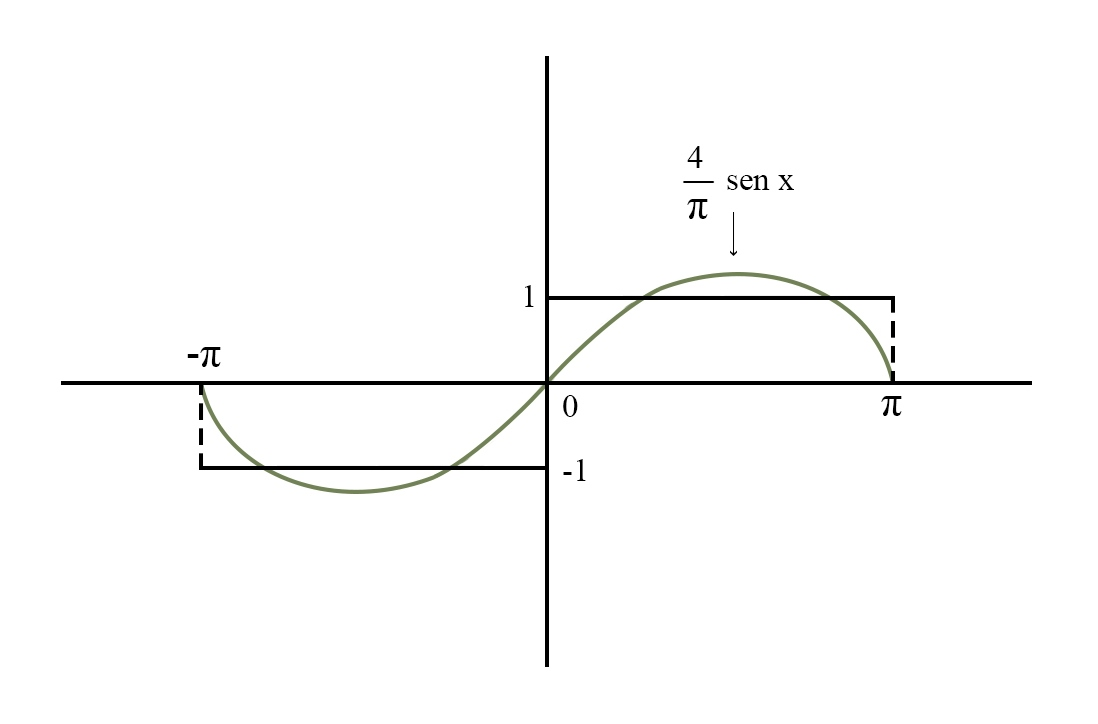
\includegraphics[width=0.8\textwidth]{Pictures/fig.38.jpg}
    \caption{Aproximación mediante un polinomio trigonométrico}
    \label{Fourier1}
\end{figure} 

\bigskip

 \begin{example}
 
 Se desea hallar la aproximación de mínimos cuadrados de $f(x)=x$  en $[0, 2 \pi]$ por medio de un polinomio trigonométrico de orden $2$ o menor.
 \begin{eqnarray}
 a_0= \frac{1}{\pi} \int_0^{2\pi} f(x)dx = \frac{1}{\pi} \int_0^{2\pi} x dx =2 \pi
 \label{90}
 \end{eqnarray}
 
 Para $k=1, 2,\cdots n $ se puede verificar que, realizando integración por partes, se obtiene
 \begin{eqnarray*}
 a_k= \frac{1}{\pi} \int_0^{2\pi} f(x)cos(kx)dx = \frac{1}{\pi} \int_0^{2\pi} x cos(kx)dx =0
 \label{91}
 \end{eqnarray*}
  \begin{eqnarray*}
 b_k= \frac{1}{\pi} \int_0^{2\pi} f(x)sen(kx)dx = \frac{1}{\pi} \int_0^{2\pi} x sen(kx)dx =\frac{-2}{k}
 \label{92}
 \end{eqnarray*}
 Por lo tanto, la aproximación de mínimos cuadrados  por medio de un polinomio trigonométrico de orden $2$ o menor es
 \[
 x \approx  \pi -2 sen(x) - sen(2x)
 \]
 \end{example}
 De lo anterior se desprende que  la aproximación de mínimos cuadrados de $f(x)=x$  en $[0, 2 \pi]$ por medio de un polinomio trigonométrico de orden $n$ o menor, teniendo en cuenta (\ref{91}), es
 \[
 x \approx  \pi -2 (sen(x) + \frac{sen(2x)}{2} + \frac{sen(3x)}{3}  + \cdots \frac{sen(nx)}{n}
 \] 
 y resulta obvio esperar que el error cuadrático medio disminuya a medida que se aumenta el número de términos en la aproximación de mínimos cuadrados
 
 \[
 f(x) \approx  \frac{a_0}{2}+ \sum_{k=1}^n (a_k cos(kx) + b_k sen(kx) ) \]
 Se puede probar que el error cuadrático medio tiende a $0$ cuando $n \rightarrow \infty$, esto se denota escribiendo
 \begin{equation}
   f(x) =  \frac{a_0}{2}+ \sum_{k=1}^\infty (a_k cos(kx) + b_k sen(kx) )  
   \label{95} 
 \end{equation}
 
 
 
 El segundo miembro de esta ecuación se denomina \textit{serie de Fourier} para $f$.
 Las series de este tipo tienen importancia primordial en ingeniería, ciencias y matemáticas.
 
 
\bigskip


\subsection{Series de Haar. Bases de wavelets ortogonales}
En la sección anterior se describió el sistema trigonométrico
\begin{equation}
   \{1, cos(nx), sen(nx)\}_{n \in N}
   \label{100}
    \end{equation}
    de período $2\pi$
a partir del cual se halla la serie de Fourier de una función $f(x)$.
Puede reescribirse con exponenciales complejas 
\begin{equation}
   \{e^{inx}\}_{n \in Z}
   \label{101}
    \end{equation}
ya que por  la fórmula de Euler,  $e^{ix}=cos(x)+ i sen(x)$. 

Los sistemas (\ref{100}) y (\ref{101})  pueden obtenerse uno del otro mediante combinaciones lineales simples.
En particular, para $n \in Z$, 
\[
e^{inx}=\left\{
\begin{array}{ll}
   cos(nx)+ i sen(nx)  & \mbox{si $n \ne 0$}, \\
    1 & \mbox{si $n = 0$}
\end{array}
\right.
\]

y para $n \in N$

\[
cos(nx)=\frac{e^{inx}+e^{-inx}}{2}
\]
y 
 \[
sen(nx)=\frac{e^{inx}-e^{-inx}}{2i}.
\]  

La serie de Fourier (\ref{95}) puede escribirse, entonces, 
\begin{equation}
   f(x) =   \sum_{k \in Z} c(k) e^{inx}  
   \label{105} 
 \end{equation} 
 con ciertos coeficientes $c(k)$.
 Vamos a presentar en esta sección un ejemplo de sistema ortogonal en $[0,1]$ conocido como \textit{el sistema de  Haar}. Es la más simple e históricamente el primer ejemplo de una base \textit{wavelet ortogonal}. Muchas de sus propiedades contrastan con las propiedades del sistema trigométrico  (\ref{101}):
 
 \begin{itemize}
     \item las funciones base de Haar tienen soporte en pequeños subintervalos de $[0,1]$, mientras que las funciones base de Fourier son no nulas en todo el intervalo $[0,1]$.
     \item las funciones base de Haar son escalonadas, con discontinuidades, mientras que las funciones base de Fourier con $C^{\infty}$ en $[0,1]$.
     \item las bases de Haar   tienen un índice que indica la escala $j$ que reemplaza  a la frecuencia $n$ de las bases de Fourier.  
     
     \item las bases de Haar proveen una representación eficiente para funciones que son suaves en algunos segmentos y con picos y discontinuidades en otros, mientras que las bases de Fourier dan buenas representaciones para funciones con comportamiento oscilatorio en intervalos largos.
     
     
 \end{itemize}


 

 \bigskip

\index{Haar, Alfréd  }
\begin{parchment}[Alfréd Haar (1885 - 1933)]{Matemático húngaro de origen judío, nacido en 1885. En 1904 comenzó a estudiar en la Universidad de Gotinga. Su doctorado fue supervisado por David Hilbert. La medida de Haar, la ondícula de Haar y la transformación de Haar reciben su nombre. Entre 1912 y 1919 enseñó en la Universidad Francisco José de Kolozsvár. Junto con Frigyes Riesz, hizo de la Universidad de Szeged un centro de las matemáticas. También fundó la revista Acta Scientiarum Mathematicarum junto con Riesz. \cite{haar} }
\end{parchment}


 \bigskip
 
 Para cada par de enteros $j$, $k$ $\in Z$, se definen 
 
 
 el \textit{intervalo diádico} $I_{j,k}$:
 \begin{equation}
   I_{j,k} = [2^{-j}k,2^{-j}(k+1)) 
   \label{108} 
 \end{equation} 
 
 y la función de Haar:
 \begin{equation}
   h_{j,k}(x) = 2^{j/2}(\chi_{I^{l}_{j,k}} (x) - \chi_{I^{r}_{j,k}} (x)  ) 
   \label{110} 
 \end{equation} 
 
 \bigskip
 
 
 De esta forma,  $h_{j,k}(x)$ está soportada en el intervalo $I_{j,k}$ (no se anula en ese intervalo). Decimos que la función de Haar $h_{j,k}(x)$ está asociada a ese intervalo.
 
 La longitud del intervalo $I_{j,k}$  es $2^{-j}$. Si $j$ es grande, la longitud es pequeña. Se dice, entonces, que  la función $h_{j,k}(x)$   \textit{está bien localizada en el tiempo}. Esta propiedad contrasta con las bases de Fourier que tienen todas módulo $1$  para todo   $x \in [0,1)$ y por lo tanto no se anulan para ningún $x$ de ese intervalo.
 
En la Figura \ref{Haar} se muestra un ejemplo de aproximación de una función mediante bases de Haar, para dos escalas, o niveles de resolución diferentes.

 \bigskip
 
\begin{figure}
    \centering
    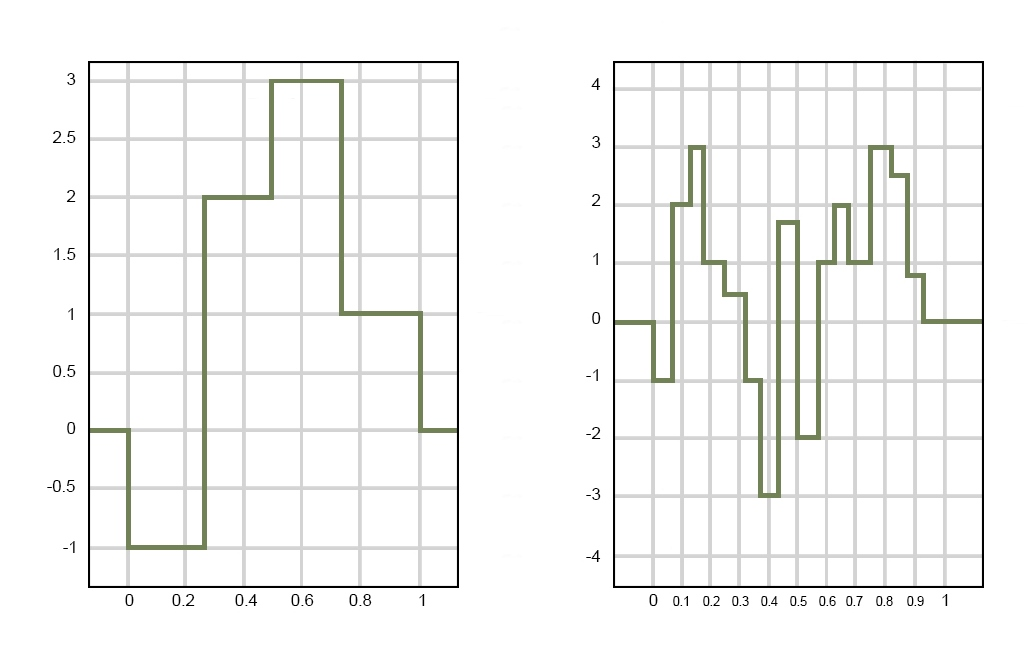
\includegraphics[width=0.8\textwidth]{Pictures/fig.37.jpg}
    \caption{Bases de Haar. Escala $j=2$ a la  izquierda y $j=4$ a la derecha.}
    \label{Haar}
\end{figure} 

\bigskip
Las bases de  Haar, creadas por Alfred Haar en 1909, fueron el primer registro histórico de lo que hoy se denomina    familias de funciones  \textit{ondículas o wavelets}  desarrolladas en los últimos 40 años  para poder analizar señales que no se comportan en forma estacionaria o que presentan cambios bruscos en intervalos pequeños. Esas señales de interés, provienen de distintas áreas como la medicina, sismología, geología, electrónica y también astronomía.
Así, la Teoría Wavelet, caracterizada por una base matemática compleja, constituye una potente herramienta en el procesamiento de señales y de imágenes digitales. Permite la reducción de ruido, la compresión de señales ( muy importante tanto para la transmisión de grandes cantidades de datos como en su almacenamiento) o la detección de determinados objetos en imágenes o en irregularidades locales, por ejemplo en un electrocardiograma (ECG).



El concepto de wavelets como lo conocemos fue propuesto por Jean Morlet y el equipo del Centro de
Física Teórica de Marsella, Francia. Con el fin de descomponer y estudiar ciertas señales sísmicas, diseñaron la wavelet que se muestra en   la Figura \ref{MORLET}.
Cabe señalar que los métodos del análisis wavelet fueron
desarrollados principalmente por Yves Meyer y sus colegas y que recién en 1988
apareció el primer algoritmo de cálculo y su autor fue Stephane Mallat.
Desde entonces
la investigación acerca del análisis Wavelet  captó mucho interés  y se
destacan científicos como Ingrid Daubechies, quien en 1988 creó una familia de  de ondículas o wavelets  ortogonales con soporte compacto. En la Figura  \ref{db6yECG} se muestra la wavelet de Daubechies de orden 6, uitilizada con frecuencia, por su similitud, para analizar electrocardiogramas, 


Su aplicación se extiende a campos muy  diversos. En cuanto a las aplicaciones en medicina, el análisis con Wavelets permite interpretar los resultados de exámenes médicos, facilitando el diagnóstico de enfermedades. 

 
%\bigskip
 
\begin{figure}
    \centering
    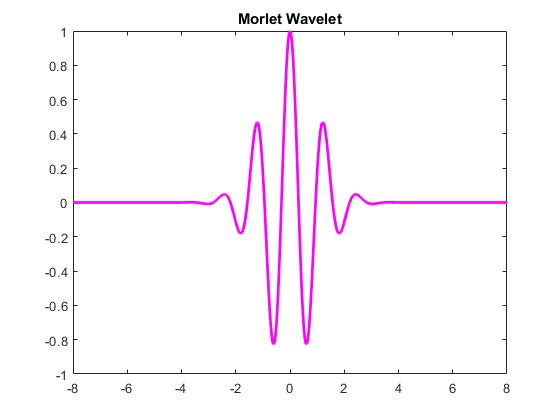
\includegraphics[width=0.8\textwidth]{Pictures/MORLET.jpg}
    \caption{Wavelet Morlet.}
    \label{MORLET}
\end{figure} 

\bigskip
\begin{figure}
    \centering
    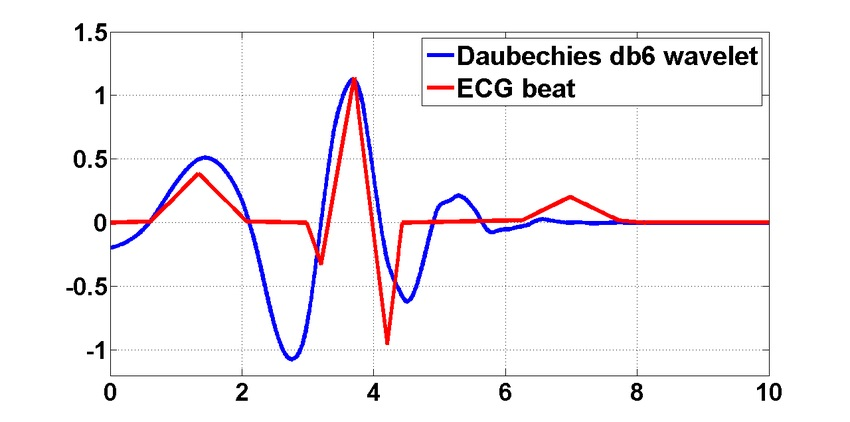
\includegraphics[width=0.9\textwidth]{Pictures/im.jpg}
    \caption{Wavelet de Daubechies y latido de un ECG. }
    \label{db6yECG}
\end{figure} 
 En Astronomía, algunos ejemplos del uso de Wavelets son:

\begin{itemize}

\item para el procesado de imágenes planetarias 

%https://www.surastronomico.com/procesado-imagenes-planetarias-2.html  (es un tutorial)

\item en el estudio de la actividad solar

\item para la detección de períodos en curvas de luz. 
%Alberici Adam, Aldana. TESIS DE GRADO FCAGLP 2022. 
        
\end{itemize}


\bigskip





 \bigskip
\index{Daubechies, Ingrid}
\begin{parchment}[Ingrid Daubechies] {Es una matemática y física belga. Nació en 1954. Estudió física en la Vrije Universiteit Brussel (la universidad de Bruselas en lengua flamenca), en la que también se doctoró en física teórica en 1980 y estuvo investigando hasta 1987. Ese año se trasladó a Estados Unidos con su marido, el también matemático Robert Calderbank, recién casados. Daubechies trabajó en los Laboratorios Bell de Nueva Jersey y en varias universidades estadounidenses. En 1993 se convirtió en profesora de matemática computacional en la Universidad de Princeton hasta 2011, cuando trasladó a la Universidad Duke como catedrática de matemáticas.
En 2012, el rey Alberto II de Bélgica la concedió el título de Baronesa en reconocimiento de su trayectoria profesional.
Es miembro de numerosas instituciones. Fue la primera mujer matemática en presidir la Unión Matemática Internacional (desde 2011). En 1993 fue admitida en la Academia Estadounidense de las Artes y las Ciencias, en 1998 en la Academia Nacional de Ciencias de Estados Unidos y en 2012 en la Sociedad Estadounidense de Matemática. Además, ha sido invitada a participar en numerosas ocasiones en el Congreso Internacional de Matemáticas.
Daubechies ha recibido numerosos premios, entre ellos destacan el Premio Nemmers en Matemáticas de 2012 y el Premio Fundación BBVA Fronteras del Conocimiento en Ciencias Básicas 2012 junto a David Mumford.
En 2020 fue reconocida, junto a Emmanuel Candès, Yves Meyer y Terence Tao, con el Premio Princesa de Asturias de Investigación Científica y Técnica por «haber realizado contribuciones pioneras y trascendentales a las teorías y técnicas modernas del procesamiento matemático de datos y señales».
En 2023 recibió el Premio Wolf en Matemáticas, por sus investigaciones sobre ondículas y análisis armónico aplicado. Daubechies es la primera mujer que ha recibido este reconocimiento.

Ingrid Daubechies ha trabajado en el campo de las ondículas, herramientas que permiten el análisis de señales para entregar información temporal y frecuencial de manera casi simultánea. En 1988, Daubechies propuso la ondícula ortogonal con soporte compacto (conocida como ondícula Daubechies), y en 1992 la ondícula biortogonal, también conocida como ondícula CDF (Cohen-Daubechies-Feauveau), empleada para el formato de compresión de imágenes JPEG 2000.
Estas herramientas matemáticas permiten el avance e investigación tanto en matemática teórica como aplicada, pues sirve en la demostración tanto de teoremas como en el desarrollo de las telecomunicaciones, tanto en audio como vídeo, y hasta el ámbito biosanitario, con transmisión de datos de imágenes sanitarias. \cite{IngridD}  }
\end{parchment}

%Ejemplos básicos de álgebra lineal con python
%https://www.redalyc.org/journal/6079/607963609005/html/